\section{Esempi di lavorazione}
Mostriamo ora alcuni esempi di lavorazione, per vedere come i tempi di esecuzione catalogati variano a seconda dei parametri scelti.

Le prove sono state effettuate usando i due file messi a disposizione per i testing, uno con oltre 7000 posizioni, e l'altro con oltre 20000. I tempi riportati si riferiscono a test effettuati usando una macchina con Ubuntu Linux 12.04 a 64 bit, con processore Intel i7 a 1.73 GHz e 4GB di RAM, con il simulatore compilato in modalità \verb!release!. Per la profilazione invece si è reso necessario compilare on modalità \verb!debug!. Abbiamo effettuato varie prove per ciascuna configurazione, e abbiamo qui riportato i valori medi.

\subsection{Modalità testuale}
Vediamo innanzitutto (tabelle \ref{tab:positionsnone} e \ref{tab:positions2none}) come si comporta il simulatore quando viene eseguito in modalità solo testuale.

\begin{center}
  \begin{table}[h]
    \begin{minipage}{.5\linewidth}
      \vspace{0pt}
      \centering
      \begin{tabular}{ccc}
        \toprule
          \shortstack{Dimensione\\ Voxel} & \shortstack{Tempo \\\texttt{[s]}} & \shortstack{Memoria \\\texttt{[MiB]}}\\
        \midrule
          3   & 0.517  & -     \\
          2.5 & 0.543  & -     \\
          2   & 1.632  & 17.2  \\
          1.5 & 1.607  & -     \\
          1   & 8.437  & 70.0  \\
          0.5 & 67.691 & 334.7 \\
        \bottomrule
      \end{tabular}
      \caption{Test con file \texttt{positions.txt}.}
      \label{tab:positionsnone}
    \end{minipage}
    \begin{minipage}{.5\linewidth}
      \vspace{0pt}\raggedright
      \centering
      \begin{tabular}{ccc}
        \toprule
          \shortstack{Dimensione\\ Voxel} & \shortstack{Tempo \\\texttt{[s]}} & \shortstack{Memoria \\\texttt{[MiB]}}\\
        \midrule
          3   & 2.446   & 22.7   \\
          2.5 & 2.558   & 12.2   \\
          2   & 11.478  & 90.6   \\
          1.5 & 11.613  & 95.0   \\
          1   & 99.785  & 463.4  \\
          0.5 & 973.191 & 2764.8 \\
        \bottomrule
      \end{tabular}
      \caption{Test con file \texttt{positions2.txt}.}
      \label{tab:positions2none}
    \end{minipage}
    %\caption{Riepilogo dei test effettuati in modalità testuale.}
    %\label{tab:graphicsnone}
  \end{table}
\end{center}

Vediamo come con voxel grandi i tempi di esecuzione sono molto ridotti e molto simili, con poca occupazione di memoria, mentre con voxel più piccoli i tempi crescono compatibilmente con un fattore 8 (l'arietà dell'Octree). Questo è segno che con voxel grandi l'albero generato è poco profondo e viene analizzato molto velocemente, con un impatto poco significativo sul tempo di esecuzione totale. Al diminuire della dimensione dei voxel, l'Octree è invece più profondo, e la sua scansione occupa una parte sempre più consistente del tempo di esecuzione totale.

Per quanto riguarda i tempi rilevati per la lavorazione del file \texttt{positions2.txt} con dimensione voxel pari a $0.5$, si segnala che la lavorazione è stata rallentata dalle operazioni di swap occorse a causa dell'elevata quantità di memoria richiesta.

\subsection{Modalità grafica \texttt{box}}
La modalità grafica \texttt{box} è la modalità che non utilizza l'algoritmo Marching Cubes per il taglio dei voxel, ma usa l'oggetto \texttt{Box} di OpenSceneGraph per rappresentare ciascun voxel.

\subsection{Modalità grafica \texttt{mesh}}
La terza modalità di visualizzazione è quella che utilizza l'algoritmo Marching Cubes per estrarre la mesh tridimensionale dai voxel.

\subsection{Confronto tra \texttt{box} e \texttt{mesh}}
Mettiamo ora a confronto la visualizzazione della lavorazione con la modalità di visualizzazione \texttt{box} e la modalità \texttt{mesh} (le immagini sono zoomate per apprezzare le differenze).
\begin{center}
\begin{table}[h]
  \begin{tabular}{cc}
   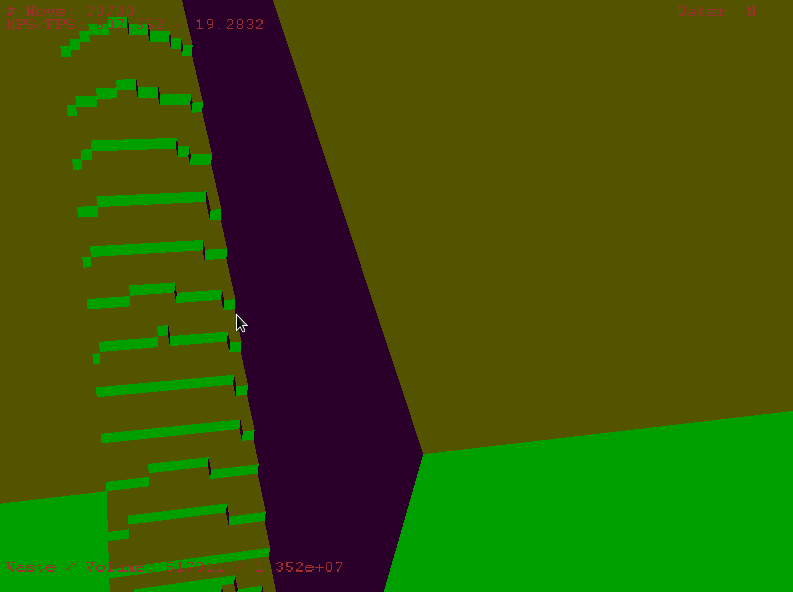
\includegraphics[width=0.48\textwidth]{img/screenshots/pos2_box_v2_2.png} &%
   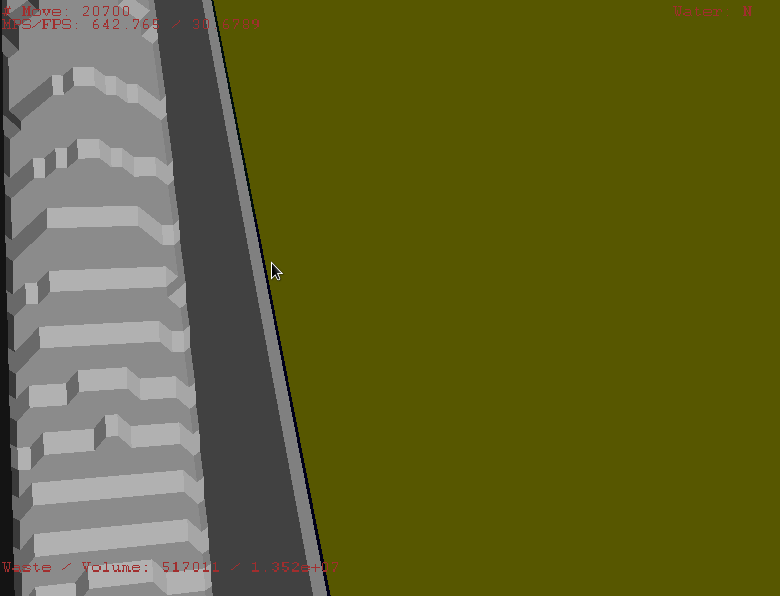
\includegraphics[width=0.48\textwidth]{img/screenshots/pos2_mesh_v2_2.png}\\
  \end{tabular}
  \caption{Confronto tra modalità \texttt{box} e modalità \texttt{mesh} con dim. voxel pari a $2$.}
  \label{tab:confrontobm1}
\end{table}
\end{center}

In \ref{tab:confrontobm1} vediamo la differenza nell'approssimazione della fresatura da parte del cilindro in modalità \texttt{box} (a sx) e \texttt{mesh} (a dx) con dimensione minima dei voxel pari a $2$. Vediamo come, nella modalità \texttt{mesh}, l'algoritmo Marching Cubes approssimi meglio la lavorazione, pur mantenendo visibile la struttura ``a cubi'' del rendering.

\begin{center}
\begin{table}[h]
  \begin{tabular}{cc}
   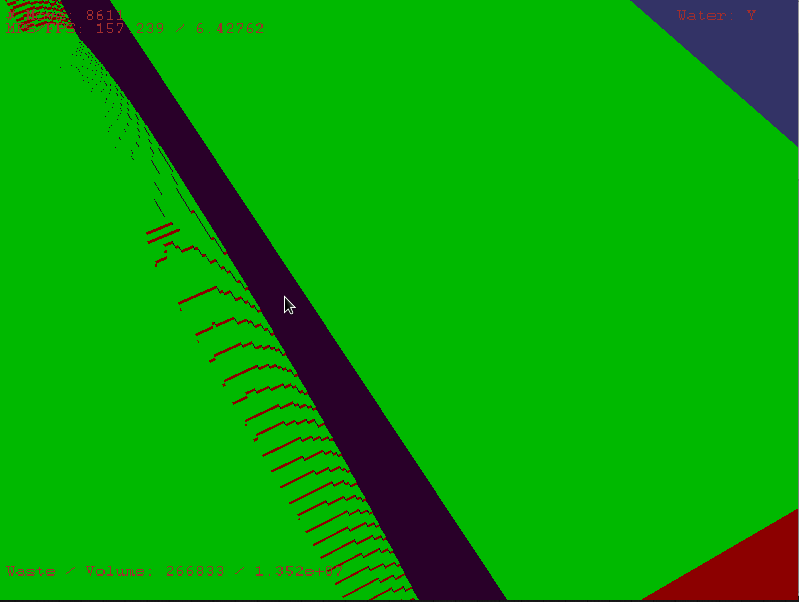
\includegraphics[width=0.48\textwidth]{img/screenshots/pos2_box_v1.png} &%
   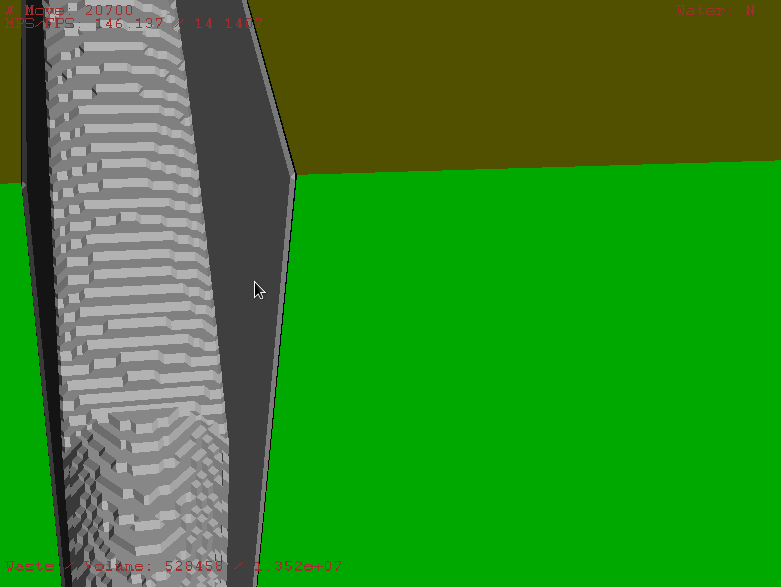
\includegraphics[width=0.48\textwidth]{img/screenshots/pos2_mesh_v1_2.png}\\
  \end{tabular}
  \caption{Confronto tra modalità \texttt{box} e modalità \texttt{mesh} con dim. voxel pari a $1$.}
  \label{tab:confrontobm2}
\end{table}
\end{center}

\begin{center}
\begin{table}[h]
  \begin{tabular}{cc}
   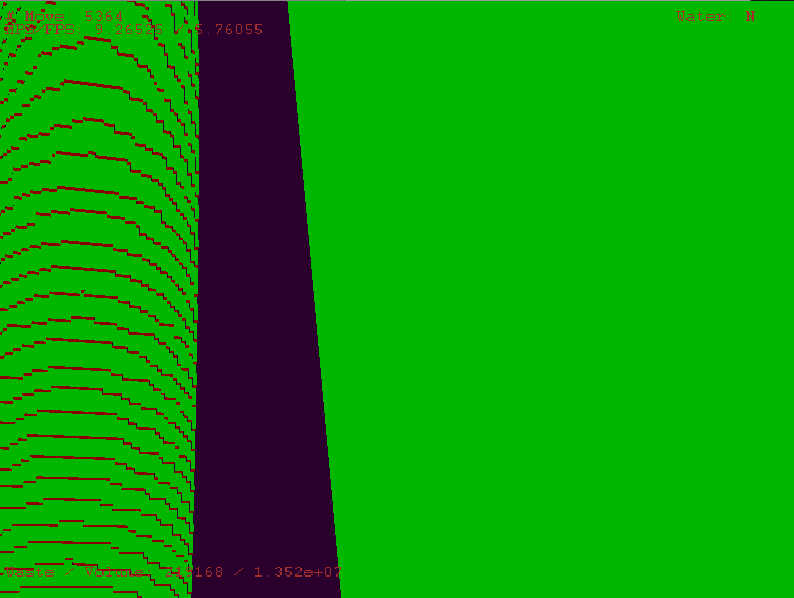
\includegraphics[width=0.48\textwidth]{img/screenshots/pos2_box_v05.png} &%
   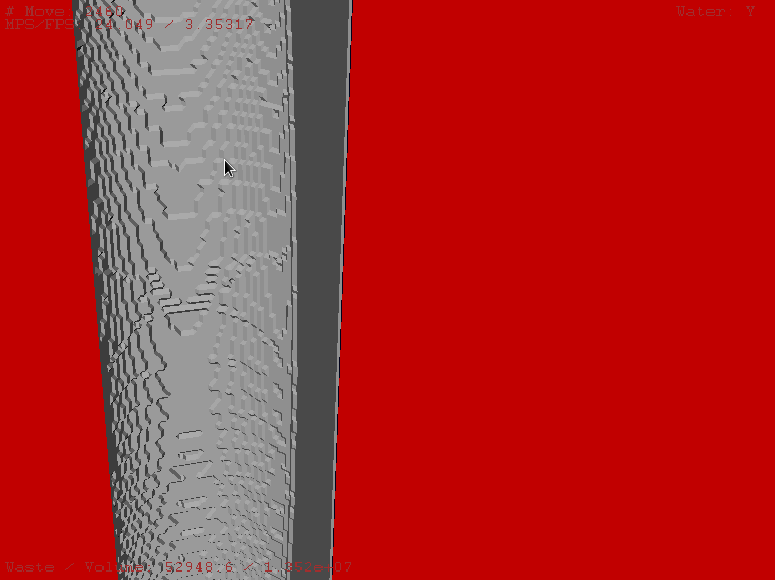
\includegraphics[width=0.48\textwidth]{img/screenshots/pos2_mesh_v05.png}\\
  \end{tabular}
  \caption{Confronto tra modalità \texttt{box} e modalità \texttt{mesh} con dim. voxel pari a $0.5$.}
  \label{tab:confrontobm3}
\end{table}
\end{center}

In \ref{tab:confrontobm2} e \ref{tab:confrontobm3} invece vediamo la stessa lavorazione, effettuata con dimensione dei voxel pari a, rispettivamente, $1$ e $0.5$. Vediamo come man mano che la dimensione dei voxel diminuisce, entrambe le modalità, ovviamente, approssimano in maniera sempre più precisa la fresatura. Tuttavia, mentre la modalità \texttt{box} approssima la lavorazione in modo sempre più preciso ma rimane comunque visibile la quadrettatura, l'algoritmo Marching Cubes che lavora alla stessa profondità dell'Octree fornisce risultati sempre più precisi e realistici.

Vediamo, invece, dalla tabella \ref{tab:confrontoBoxMesh} come l'implementazione con Marching Cubes sia più veloce, seppur di poco, in lavorazioni veloci e che comportino la generazione di un Octree poco bilanciato e poco profondo. All'aumentare della profondità dell'albero, invece, la semplicità della generazione dei \texttt{Box} di OSG risulta più veloce. Per lavorazioni più complesse, che richiedono un Octree più completo, l'approccio \texttt{box} è più veloce rispetto alla generazione della \texttt{mesh} in tutti i test effettuati.

Segnaliamo che, per dimensioni del voxel sufficientemente grandi, la lavorazione termina in tempi talmente brevi che risulta impossibile misurare un tempo attendibile, per questo.

\begin{center}
  \begin{table}[h]
   \centering
      \begin{tabular}{cccccc}
        \toprule
        & \multicolumn{2}{c}{file \texttt{positions.txt}} & & \multicolumn{2}{c}{file \texttt{positions2.txt}}\\
        \cmidrule(r){2-3}\cmidrule(r){5-6}
          \shortstack{Dimensione\\ Voxel} & \shortstack{Tempo \\con \texttt{box} \texttt{[s]}} & \shortstack{Tempo \\con \texttt{mesh} \texttt{[s]}} & & \shortstack{Tempo \\con \texttt{box} \texttt{[s]}} & \shortstack{Tempo \\con \texttt{mesh} \texttt{[s]}}\\
        \midrule
          3   & -      & -      & & 2.381    & 2.690    \\
          2.5 & -      & -      & & 2.510    & 2.581    \\
          2   & 2.090  & 1.988  & & 12.719   & 16.221   \\
          1.5 & 2.093  & 1.971  & & 12.581   & 19.051   \\
          1   & 10.267 & 9.807  & & 126.827  & 127.073  \\
          0.5 & 81.466 & 94.821 & & arriva.. & 1684.734 \\
        \bottomrule
      \end{tabular}
      \caption{Confronto delle prestazioni tra modalità \texttt{box} e \texttt{mesh}.}
      \label{tab:confrontoBoxMesh}
  \end{table}
\end{center}

\subsection{Carico relativo dei moduli}
Analizziamo ora cosa succede \textit{all'interno} di un'esecuzione del simulatore. Per farlo, osserviamo il grafico delle chiamate in figura \ref{fig:callgraph}. Questo grafico è stato ottenuto a partire dal una lavorazione in modalità \texttt{mesh} con dimensione dei voxel pari a $2$, con gli strumenti di debug e profiling \texttt{valgrind}, \texttt{callgrind} e \texttt{kcachegrind}.

\begin{figure}[htp]
	\centering
	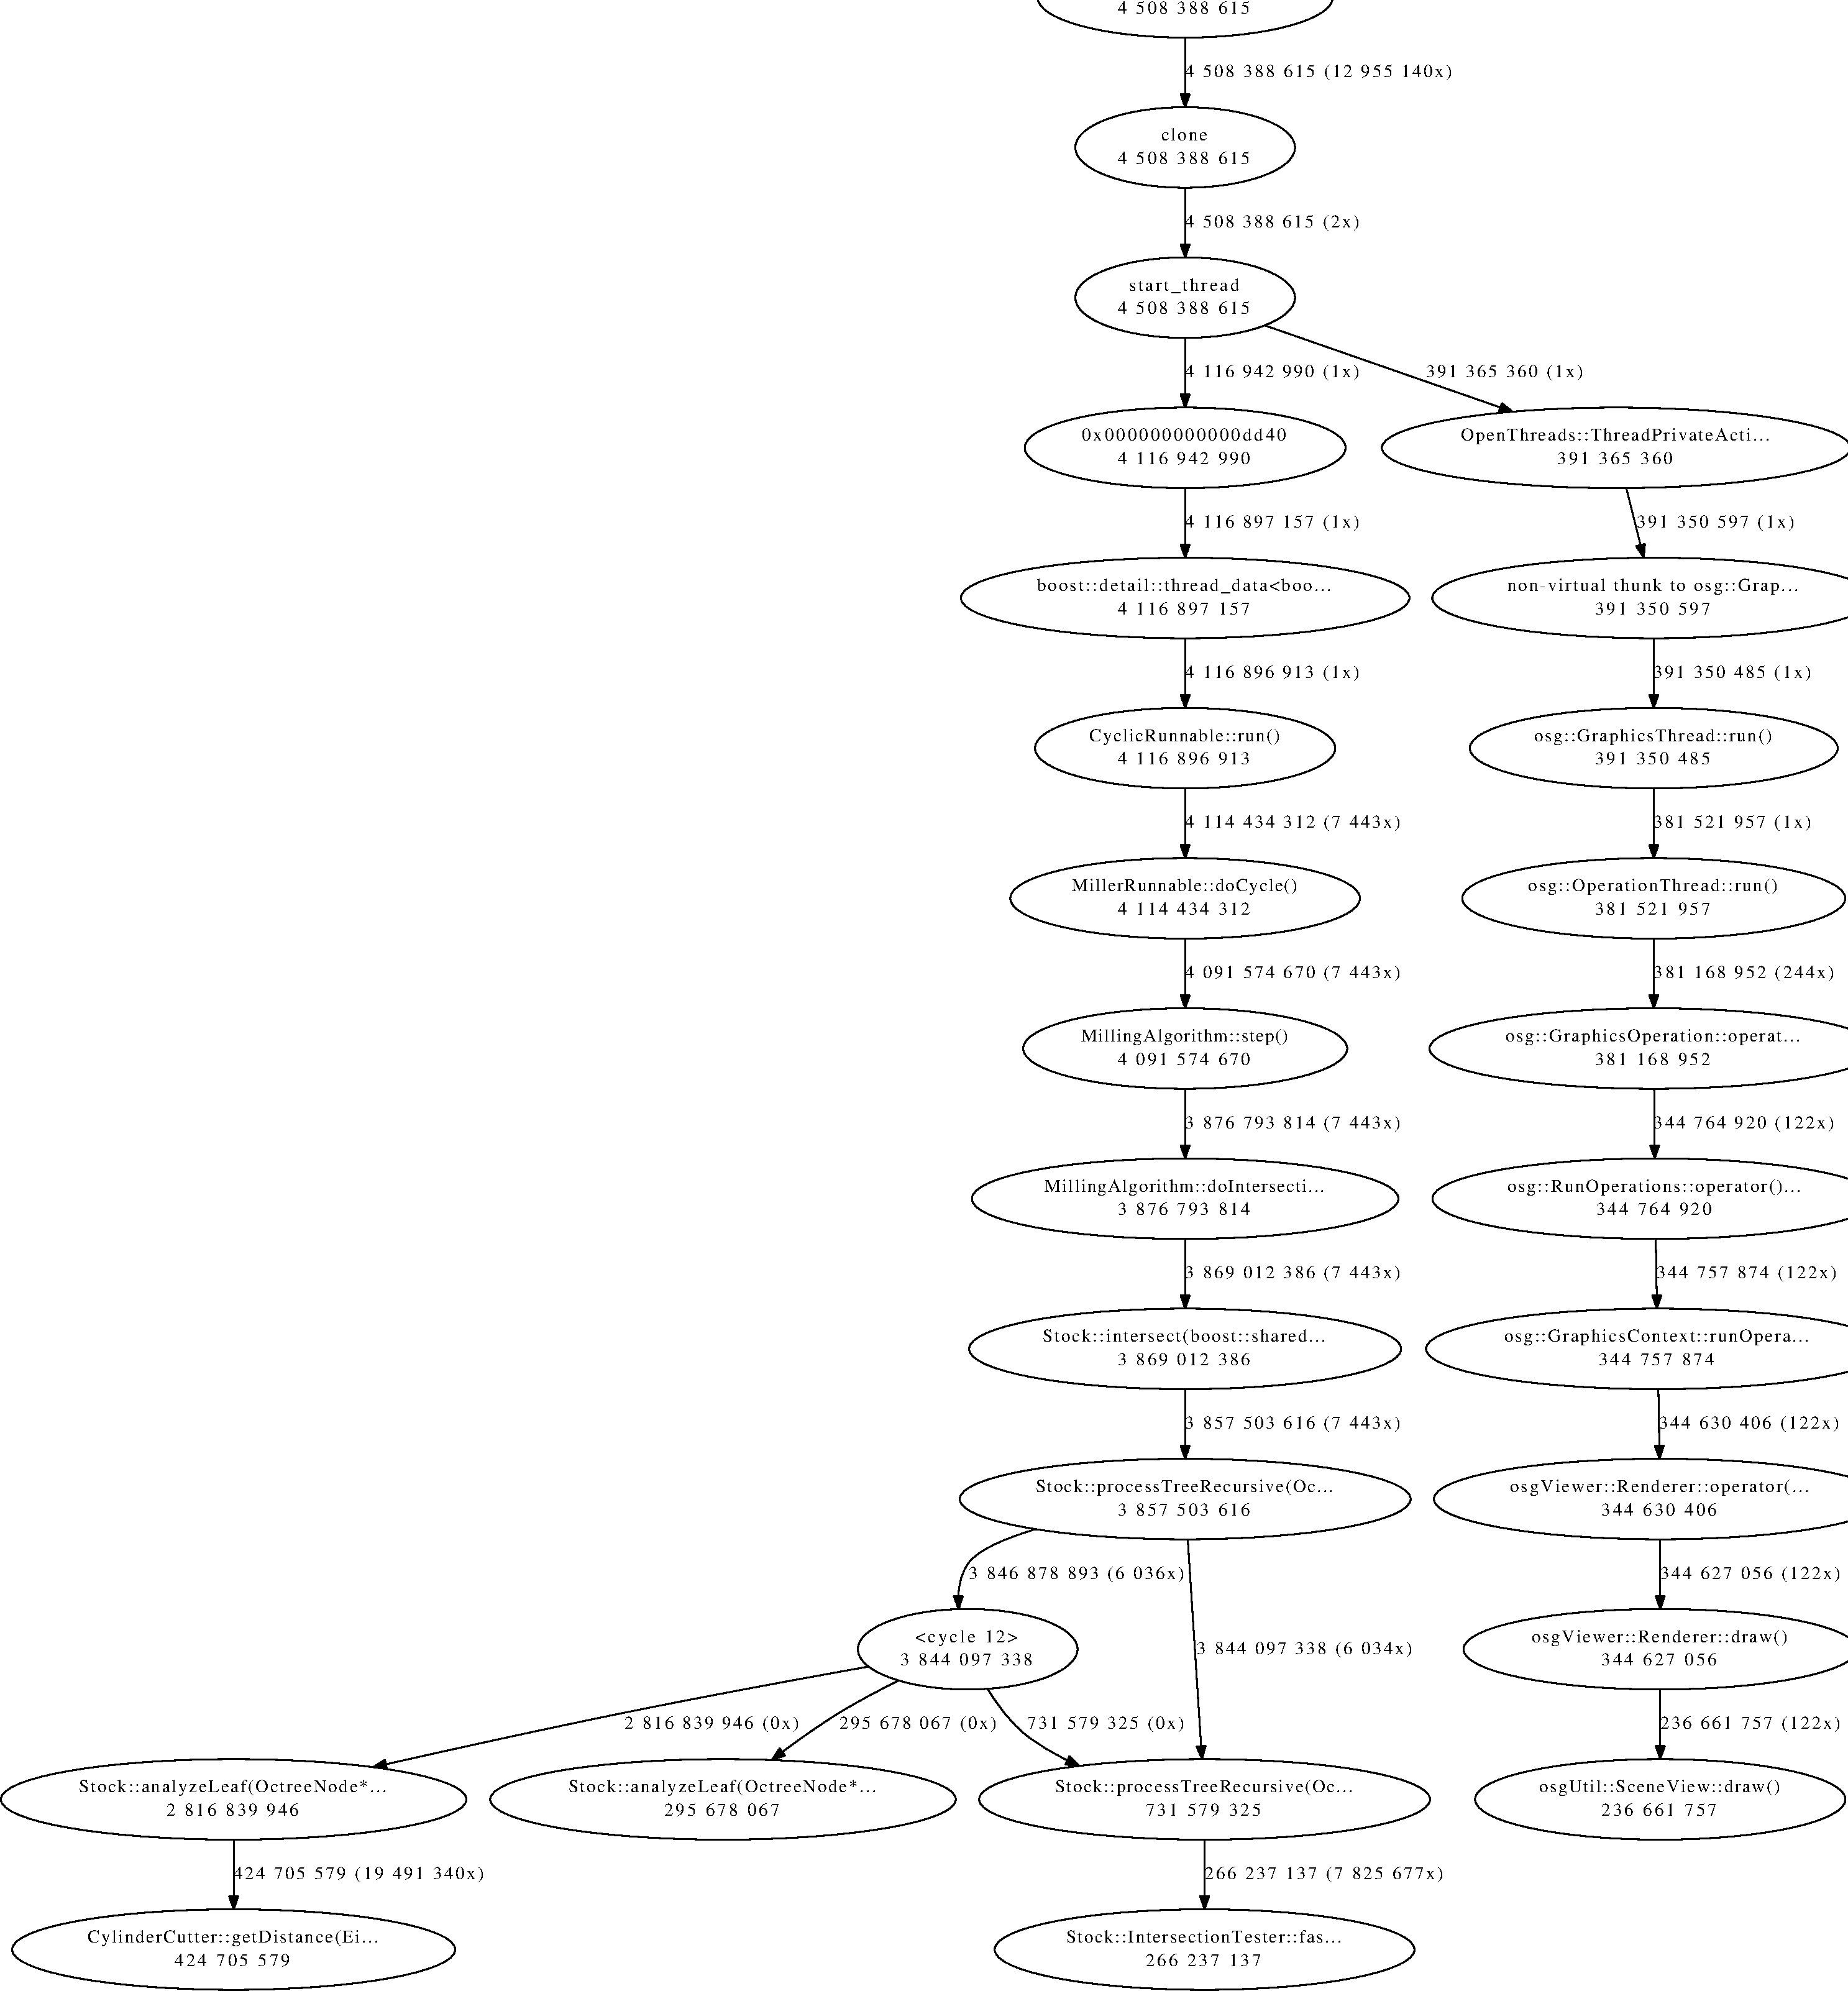
\includegraphics[width=.97\textwidth]{./img/callgraph.pdf}
	\caption{Grafico delle chiamate del simulatore.}
	\label{fig:callgraph}
\end{figure}

Il modulo che lavora per la maggior parte del tempo è chiaramente il Miller, che consuma circa i 3/4 di cicli processore impiegati in totale. Il metodo \texttt{CyclicRunnable::run()} chiama infatti \texttt{MillerRunnable::doCycle()} per 7443 volte, ovvero il numero di iterazioni dell'algoritmo di milling. Questa è chiaramente l'operazione più onerosa eseguita dall'algoritmo, e quella in cui si dovrebbero concentrare eventuali sforzi di ottimizzazione per ottenere un prodotto più performante.

La visualizzazione grafica, che inizia con l'invocazione del metodo \texttt{Display::draw()} è invece responsabile del 15\% circa del tempo di calcolo.

Per quanto riguarda i rimanenti moduli, se il configuratore viene eseguito solo preliminarmente alla lavorazione e con compiti di setup, e ci aspettiamo quindi un impatto limitato sul tempo totale, notiamo invece come il Meshing sia assente dal grafo, segno di come anche il suo impatto sia limitato rispetto al Milling, conseguenza dell'efficienza dell'algoritmo Marching Cubes e della bontà della sua implementazione.

%\subsubsection{Carico dei metodi}
Come si può facilmente evincere dai risultati appena presentati, i metodi che vengono maggiormente invocati sono quelli che permettono l'interazione tra cutter e Octree. Il metodo in assouto più chiamato è infatti \texttt{CylinderCutter::getDistance()} che misura la distanza tra il cutter (che in tutti i test effettuati era appunto di forma cilindrica) e il voxel più vicino, per determinare se c'è intersezione e quindi rimozione di materiale. Segue, con circa metà invocazioni, la gestione degli smart pointers di Boost e, con poco più di un terzo di chiamate, il metodo \texttt{Stock::IntersectionTester::fastInt()} che esegue i calcoli per determinare se c'è intersezione tra cutter e voxel.
